We consider the 2D base flow shown on Figure \ref{khappfig}. Coordinates are noted $(x,z)$ and vectors
$(u,w)$. The height of the interface is $h(x,t)$. The flow has density $\rho_1$ for $z<h(x,t)$ and 
$\rho_2$ for $z>h(x,t)$ and is incompressible. The base flow is a parallel shear flow.
The base flow is uniform with $u=-U$ for $z<0$
and $u=U$ for $z>2a$, with a linear (Couette flow) boundary layer in between.  When $\rho_1 \neq \rho_2$ the heavier fluid is the ``liquid'' and the lighter the ``gas''. For $\rho_1 > \rho_2$ the boundary layer is in the gas while otherwise the bounary layer is in the liquid. 
Similar flows have been studied
in \cite{Matas_2011a,Eggers08}.

\begin{figure}
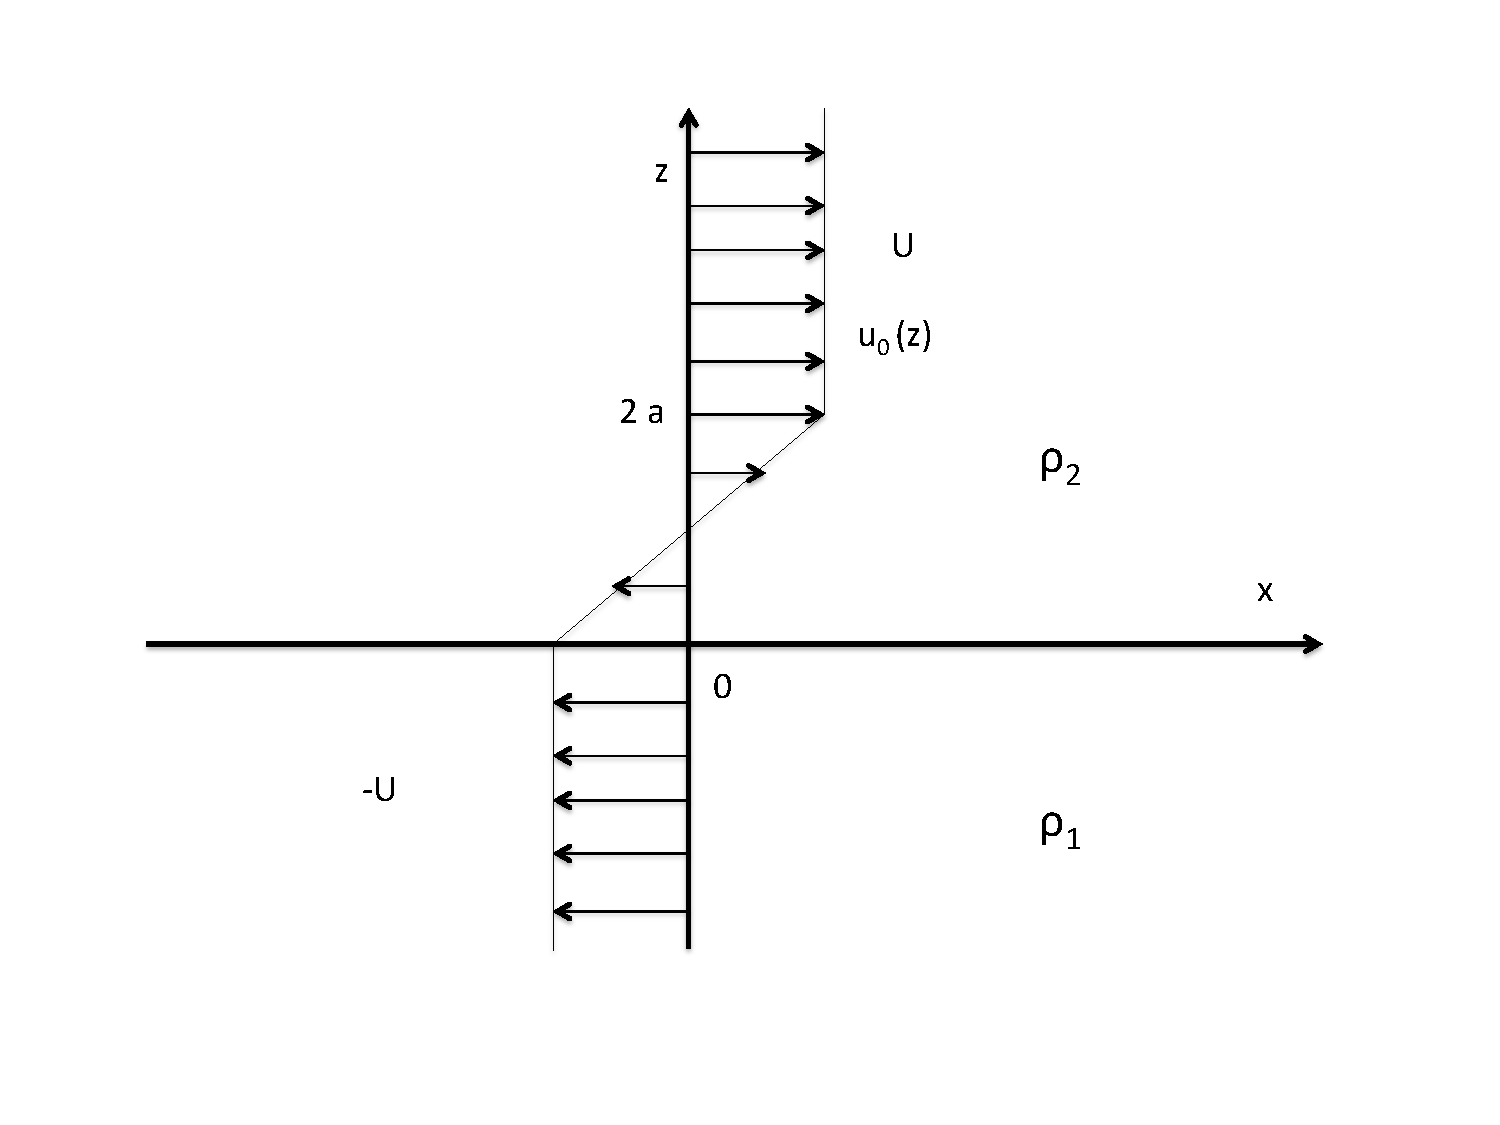
\includegraphics[width=0.8\textwidth]{Figures/2-1.pdf}
\caption{Base velocity profile. \label{khappfig} }
\end{figure}

\subsection{Dispersion relation}

The Euler and incompressibility 
equations are as in Eqs. (\ref{nse1}) with only
$
\LLL =  \LLL_{\rm conv} 
$, surface tension and viscosity are not included.
The interface height $h$ moves according to
\be
\dert h +  u \derx h =  w \label{heq}
\nd
We also use a stream function $\psi$
\be
w = - \derx \psi, \quad u = \dery \psi \label{psiu}
\nd
We consider a small perturbation of the base velocity 
in the form
\be
\U = \U_0  + \eps \U_1 + {\cal O}(\eps^2) \label{1}
\nd
the pressure expands as 
$p=p_0 + \eps p_1(x,z,t) + {\cal O}(\eps^2)$, the height as
$h= \eps h_1(x,z,t) + {\cal O}(\eps^2)$,
and similarly
the stream function. 
We assume the following form for the perturbation
\be
\left(
\ba{c} u_1 \\ w_1 \\ p_1 \\ \psi_1 \\ h_1 \ea \right)
=
\left(
\ba{c} U_1(z) \\ W_1(z) \\ P_1(z) \\ \Psi_1(z) \\ A_h \ea
\right)
e^{- \ii k x - \ii \om t}
\label{UVWdef} \nd
where $k$ is an  arbitrary wavenumber and $\om$ a frequency
to be determined.
Although the expressions on the rhs in (\ref{UVWdef}) are complex we understand the real part.

It is convenient to define
as Chandrasekhar \cite{Chandrasekhar} the reduced wavenumber  $\kappa = 2ka$
and the reduced frequency $\Omega=\om a/U$, which are related by 
\be
e^{-2\kappa} 
=  (1 - 2\Omega - \kappa)\frac{2 + (r+1)(2\Omega - \kappa) }{2+ ({r-1}) (2\Omega - \kappa)},
\label{ev}
\nd
see for example \cite{Eggers08}, equation (135).
The system is unstable whenever Eq. (\ref{ev}) has two complex conjugate non-real roots. Then the positive
imaginary part 
$\Omega_i$ is the growth rate, plotted on Figure \ref{gg1} in the case $r=100$
where $r={\rm max}(\rho_1/\rho_2,\rho_2/\rho_1)$.
The case $r=100$ corresponds to the boundary layer in the gas
and is much less unstable than the case with the boundary layer in the liquid. As the ratio $r$ is increased
the growth rate for the boundary layer in the gas decreases steadily while the growh rate for the boundary layer in the liquid converges to the one for a free surface, with the gas replaced by a void. 
\begin{figure}
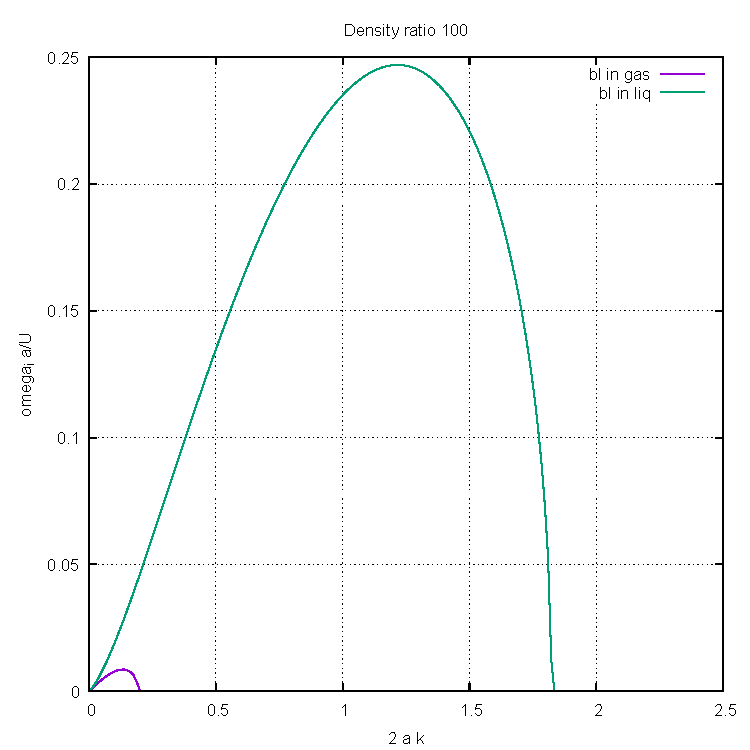
\includegraphics[width=0.8\textwidth]{Figures/rrates_100.pdf}
\caption{Growth rate for $r=100$.  \label{khappfig} }
\end{figure}

\subsection{Special case}

When $a=0$ the above is singular and a special computation
is needed. One has $\kappa=0$ and the frequencies are
\red{
  \be
\om =\left( \frac{r-1}{r+1} +\frac{2 \sqrt r}{r+1}  \ii  \right){ k U } \label{omkaz}
\nd
}

\subsection{Construction of the unstable mode}

We want to write the solution using the stream function $\psi$
in order to have a divergence free initial condition in the computations. 
The construction of $\psi$ is done by determining the relevant coefficients
so that $\psi$ is given by
\blue{
\bea
z<0 & \psi(x,z,t) & =  A_1 e^{kz} e^{-\ii k x - \ii \om t } \label{psi1} \\ 
0 <z< 2a & \psi(x,z,t) & = ( A_0 e^{kz} +  B_0 e^{-kz})  e^{-\ii k x - \ii \om t }  \label{psi2} \\
2a<z & \psi(x,z,t) &=  B_2 e^{-kz}  e^{-\ii k x - \ii \om t } \label{psi3}
\nda
}
From (\ref{heq}) 
\be
\dert h =  -U_0(0) \derx h + w \label{htw}
\nd
and from \refeq{psiu} and  \refeq{psi2} 
we get
$$
- \ii \om  A_h = -\ii k U  A_h +  \ii k (A_0 + B_0)
$$
hence
$$
(- \ii \om + \ii k U)  A_h =  \ii k (A_0 + B_0)
$$
and
$$
A_h = - \frac{k}{\om-kU} (A_0 + B_0) 
$$
Similar relations are obtained from the requirements of continuity of pressure
and normal velocity at $z=0$ and $z=2a$. 
We can then determine all the amplitudes of the constructed solution
after an amplitude for the interface has been chosen. Typically
the modulus $|A_h|$  and the argument $\phi$ are selected so that
$$A_h = | A_h | e^{\ii \phi}$$
then for $\kappa>0$ we have
\red{
\bea
C_0 & = & - (\frac{\om}k- U)A_h ( e^{-2\kappa}  +  2\Omega + \kappa - 1 )^{-1} \label{AhC0}\\
A_0 &=& C_0  e^{-2\kappa}\\
B_0 &=& C_0 (2\Omega + \kappa - 1 ) \label{AB0sol}\\
A_1 & = &  A_0 + B_0 \label{A1A0B0}  \\
B_2 & = &  A_0  e^{2 \kappa} + B_0  \label{B2A0B0}
\nda
}
These expressions for the amplitudes together with (\ref{psi1}-\ref{psi3}) are used to
initialize the stream function. The intermediate constant $C_0$ is used to simplify the expressions.

\subsection{Special cases: mode structure for $ka \rightarrow 0$}

\subsubsection{Mode structure for $a>0$ in the limit $a \rightarrow  0$.}

For small or vanishing $a$ and $\kappa$ however the expression \refeq{AhC0} is singular.
Indeed in the limit $\kappa \rightarrow 0$ we also have $\Omega \rightarrow 0$ and
$$
e^{-2\kappa}  +  2\Omega + \kappa - 1 = - 2\kappa + 2\kappa^2 +   \kappa + \Order(\kappa^3) = - \kappa + \Order(\kappa^2)
$$
and then $A_0$ and $B_0$ become spurious as the region $(0,2a)$ vanishes.
From \refeq{AhC0}
$$
C_0 \simeq  - \frac{\om}k  \frac 1 \kappa A_h
$$
and from \refeq{AB0sol}  and  \refeq{B2A0B0} 
$$
B_2 = C_0 (2\Omega + \kappa) \simeq  C_0 \kappa
$$
Thus for $a=0$
\red{
$$
B_2 = - \frac{\om}k  A_h
$$
$$
A_1 =  \frac{\om}k A_h
$$
}
the latter being obtained directly from \refeq{A1A0B0}. Since $B_2 \neq A_1$
there is a $\Order(\eps)$ discontinuity of $\psi$ which results in a jump of $v(x,z,t)$
accross the interface at $z=0$ and a related thin jet $u_1(x,z,t) \simeq \epsilon f(x,t) \delta(z)$.
This is a consequence of placing the interface in the above calculations at $z=0$ instead of
$z=\eps h_1(x,t)$ and it conflicts with the solution obtained classically with the
thin vortex sheet setup (that is, the setup in which $a=0$ is postulated at the beginning). 

\subsection{Mode structure in the $a=0$ case}

We now obtain the mode structure for the classic thin vortex sheet setup. 
In that case we keep only the terms in \refeq{w1} and \refeq{w3}. The velocity continuity condition becomes
\be
h_t = - u h_x + w = - u_0 h_x + w_1 + \Order(\epsilon) \label{ht}
\nd
which replaces \refeq{htw}. Since $h_t$ must have the same expression above and below the interface
\be
[ w  -  h_x u_0 ]=0
\nd
thus $ [ w] = h_x [u_0] = 2 h_x U $ and from  \refeq{w1} and \refeq{w3}
\bea
z<0 & W_1 &= A^\prime_1 e^{kz}  \\ 
z > 0 & W_1 &= B^\prime_2 e^{-kz}
\nda
and from \refeq{ht}
\bea
A^\prime_1 &=&  -\ii (\om - kU) A_h \label{apht}\\
B^\prime_2 &=&  -\ii (\om + kU) A_h \label{bpht}\\
\nda
The pressure equality at $z=0$ leads to
\bea
z<0 &  P_1 &=    \frac{\ii \rho_1}{k^2} (\om - kU) A^\prime_1 k e^{kz}  \\ 
z>0 &  P_1 &=    \frac{\ii \rho_2}{k^2} (\om + kU) B^\prime_2 (- k e^{-kz}) 
\nda
hence introducing $\nu = \om/(kU)$
and from  \refeq{apht} and \refeq{bpht}
\bea
(\nu+1)A_1 - (\nu-1)B_2 & = &0\\
r (\nu-1)A_1 + (\nu + 1)B_2 & = &0\\
\nda
from which one obtains
  \be
\nu = \frac{r-1}{r+1} +\frac{2 \sqrt r}{r+1}  \ii 
\nd
identical to \refeq{omkaz}. Also from \refeq{apht} and \refeq{bpht}
\bea
A_1 &=&    (U - \om/k) A_h \label{aha}\\
B_2 &=&  - (U + \om/k)  A_h \label{ahb}
\nda
These expressions should be used whenever $a \ll A_h$ while the full expressions with the boundary layer
would be valid for  $A_h \ll a$. In both cases $\Delta x \ll {\rm min}(A_h,a)$ may be required. 

